\documentclass{scrartcl}
\usepackage[utf8]{inputenc}
%\usepackage[T1]{fontenc}
\usepackage[a4paper, left=2.5cm, right=2.5cm, top=2.5cm, bottom=4cm]{geometry}
\usepackage[english]{babel}
\usepackage{amsmath, amsthm, amssymb, amstext}
\usepackage{listings}
\usepackage{color}
\usepackage{graphicx}
\usepackage{xparse}
\usepackage{fancyhdr}
\usepackage{algorithmicx}
\usepackage{algpseudocode}
\usepackage{algorithm}
\usepackage{parskip}
\usepackage[table]{xcolor}
\usepackage{tabularx}
\usepackage{enumerate}
\usepackage{enumitem}
\usepackage{float}
%\usepackage{minted}
\usepackage {tikz}
\usetikzlibrary{positioning}
\usepackage{marvosym}

\pagestyle{fancy}


\rhead{{\newcommand\and\\\getauthors}}
\author{Felix Bühler\\2973410 \and Clemens Lieb\\3130838 \and Steffen Wonner\\2862123 \and Fabian Bühler\\2953320}
\lhead{\textbf\gettitle}
\title{\gettitle}
\chead{\getsubtitle}
\subtitle{\getsubtitle}

\addtolength{\headheight}{2\baselineskip}
\renewcommand{\headrulewidth}{0pt}

\newcommand{\gettitle}{Distributed systems I\\Winter Term 2019/20}
\newcommand{\getsubtitle}{G2T1 – Assignment 6 (theoretical part)}
\newcommand{\getauthors}{Felix Bühler \and Clemens Lieb \and Steffen Wonner \and Fabian Bühler}
\setlength{\headheight}{53pt}

\begin{document}
\maketitle

\section*{1 - Replication with Atomic Multicast}

\subsection*{a)}

As shown in figure \ref{fig:1a} message M1 is delivered by R1 but not R2.
This can happen if the sender is faulty as the validity property is only enforced for correct senders.
If the agreement property is not enforced R2 may never receive the message M1.
This means that x is not replicated and R2 has a stale value even though it is still correct.

R2 will however not deliver any other message since it still expects a message with the sequence number of M1 to arrive before delivering any message with a higher sequence number.

\begin{figure}[!ht]
    \centering
    \begin{tikzpicture}[deliver/.style={fill=black,circle, inner sep=0pt, minimum size=5pt}, label/.style={font=\scriptsize}, msg/.style={->}]
    \node (C1) {C1};
    \node[below=1cm of C1] (R1) {R1};
    \node[below=1cm of R1] (R2) {R2};
    
    \node[right=6cm of C1] (C1end) {};
    \node[right=6cm of R1] (R1end) {};
    \node[right=6cm of R2] (R2end) {};
    
    \path[draw, ->]
        (C1) edge (C1end)
        (R1) edge (R1end)
        (R2) edge (R2end)
        ;
    
    \node(m1s) [right=0.5cm of C1] {};
    \node[deliver] (m1r1) [right=2cm of R1] {};
    \node[] (m1r2) [below=0.5cm of m1r1] {\Lightning};
    \node[] (fault) [right=0.5cm of m1s] {\Lightning};
    
    \path (m1s.center) edge[msg] node[label] {M1 = write(x)} (m1r1);
    \path (m1s.center) edge[msg] (m1r2);
    
    \end{tikzpicture}
    \caption{Atomic Multicast without Agreement}
    \label{fig:1a}
\end{figure}


\subsection*{b)}

Assuming the atomicity property is the total order property from the lecture.

As seen in figure \ref{fig:1b} if the total order of messages is not enforced the actual order messages are delivered at each replica may be different.
Now both replicas have a different value for x.

\begin{figure}[!ht]
    \centering
    \begin{tikzpicture}[deliver/.style={fill=black,circle, inner sep=0pt, minimum size=5pt}, label/.style={font=\scriptsize}, msg/.style={->}]
    \node (C1) {C1};
    \node[below=1cm of C1] (C2) {C2};
    \node[below=1cm of C2] (R1) {R1};
    \node[below=1cm of R1] (R2) {R2};
    
    \node[right=6cm of C1] (C1end) {};
    \node[right=6cm of C2] (C2end) {};
    \node[right=6cm of R1] (R1end) {};
    \node[right=6cm of R2] (R2end) {};
    
    \path[draw, ->]
        (C1) edge (C1end)
        (C2) edge (C2end)
        (R1) edge (R1end)
        (R2) edge (R2end)
        ;
    
    \node(m1s) [right=0.5cm of C1] {};
    \node[label] (M1) [below=0.5cm of m1s.east] {M1 = write(x)};
    \node[deliver] (m1r1) [right=4cm of R1] {};
    \node[deliver] (m1r2) [right=1.5cm of R2] {};
    
    \path (m1s.center) edge[msg] (m1r1);
    \path (m1s.center) edge[msg] (m1r2);
    
    \node(m2s) [right=1.3cm of C2] {};
    \node[label] (M2) [below right=0.5cm and -0.3cm of m2s] {M2 = write(x)};
    \node[deliver] (m2r1) [right=2.5cm of R1] {};
    \node[deliver] (m2r2) [right=5cm of R2] {};
    
    \path (m2s.center) edge[msg] (m2r1);
    \path (m2s.center) edge[msg] (m2r2);
    
    \end{tikzpicture}
    \caption{Atomic Multicast without Atomicity/Total Order}
    \label{fig:1b}
\end{figure}


\subsection*{c)}

\subsubsection*{i.}
As seen in figure \ref{fig:1c} if the client does not wait for an acknowledgement for its messages a newer message may get overwritten by an older message that was not yet delivered.
The total order property only guaranties that the order of delivered messages is the same for all replicas.

\begin{figure}[!ht]
    \centering
    \begin{tikzpicture}[deliver/.style={fill=black,circle, inner sep=0pt, minimum size=5pt}, label/.style={font=\scriptsize}, msg/.style={->}]
    \node (C1) {C1};
    \node[below=1cm of C1] (R1) {R1};
    \node[below=1cm of R1] (R2) {R2};
    
    \node[right=6cm of C1] (C1end) {};
    \node[right=6cm of R1] (R1end) {};
    \node[right=6cm of R2] (R2end) {};
    
    \path[draw, ->]
        (C1) edge (C1end)
        (R1) edge (R1end)
        (R2) edge (R2end)
        ;
    
    \node(m1s) [right=0.5cm of C1] {};
    \node[label] (M1) [below=0.3cm of m1s.east] {M1 = write(x)};
    \node[deliver] (m1r1) [right=4cm of R1] {};
    \node[deliver] (m1r2) [right=5cm of R2] {};
    
    \path (m1s.center) edge[msg] (m1r1);
    \path (m1s.center) edge[msg] (m1r2);
    
    \node(m2s) [right=2cm of C1] {};
    \node[label] (M2) [below right=0.1cm and -0.3cm of m2s] {M2 = write(x)};
    \node[deliver] (m2r1) [right=3cm of R1] {};
    \node[deliver] (m2r2) [right=3cm of R2] {};
    
    \path (m2s.center) edge[msg] (m2r1);
    \path (m2s.center) edge[msg] (m2r2);
    
    \end{tikzpicture}
    \caption{Atomic Multicast without synchronous clients}
    \label{fig:1c}
\end{figure}

\subsubsection*{ii.}

As causal atomic multicast also includes fifo ordering the wrong arrival order of messages when sending them asynchronously like in figure \ref{fig:1c} cannot happen.
Messages from the same sender will arrive in the order they were sent.

\section*{2 - Multicast Semantics}

\subsection*{a)}

\subsubsection*{i.}
False\\
m$_3$ is delivered to P$_$2 but not to P$_1$ and P$_3$ which are correct.
\subsubsection*{ii.}
True\\
m$_1$, m$_2$ and m$_4$ are send by correct processes and delivered exactly once by P$_1$ and P$_3$
\subsubsection*{iii.}
True\\
Only P$_1$ sends more than 1 messaage. The second one is send after all processes recieved the first one. So it is FIFO multicast.\\
P$_1$ and P$_2$ are delivering m$_1$ and m$_2$ in diffrent orders. So no atomic multicast.
\subsubsection*{iv.}
False\\
P$_2$ does not deliver m$_1$ but m$_4$, that violates Uniform FIFO.
\subsection*{b)}

\subsubsection*{i.}
Reliable Multicast: fullfilled\\
FIFO Multicast: violated\\
Causal Multicast: violated\\
Atomic Multicast: violated\\
\subsubsection*{ii.}
Reliable Multicast: violated\\
FIFO Multicast: violated\\
Causal Multicast: violated\\
Atomic Multicast: violated\\
\subsubsection*{iii.}
Reliable Multicast: fullfilled\\
FIFO Multicast: fullfilled\\
Causal Multicast: fullfilled\\
Atomic Multicast: violated\\
\section*{3 - Causal Mulitcast}

\subsection*{a)}
\subsubsection*{i.}
See figure \ref{fig:3a}

\begin{figure}[!ht]
	\centering
	\begin{tikzpicture}
	\draw[->, thick] (0, 6) -- (12, 6);
	\draw[->, thick] (0, 3) -- (12, 3);
	\draw[->, thick] (0, 0) -- (12, 0);
	
	\foreach \t/\p in {1/6,2/3,3/0} {
		\draw node at (-0.5, \p) {\(P_\t\)};
	};

	\draw[->, thick] (0.5, 6) -- node[pos=0.1, right] {$ m_1 $} (6, 0);
	\draw[->, thick] (0.5, 6) -- (1, 3);
	
	\draw[->, thick] (2.5, 3) -- (5, 6);
	\draw[->, thick] (2.5, 3) -- node[pos=0.3, left] {$ m_2 $} (4, 0);
	\draw[->, blue, thick] (4, 0) to [out=30,in=150] (7, 0);
	
	\draw[->, thick] (6.5, 3) -- node[pos=0.3, left] {$ m_3 $} (11, 6);
	\draw[->, thick] (6.5, 3) -- (10, 0);
	
	\draw[->, thick] (8, 0) -- (9.5, 3);
	\draw[->, thick] (8, 0) -- node[pos=0.1, left] {$ m_4 $} (9.5, 6);
		
	\draw node at (0.5, 6.3) {$ [1,0,0] $};
	\draw node at (5, 6.3) {$ [1,1,0] $};
	\draw node at (9.5, 6.3) {$ [1,1,1] $};
	\draw node at (11, 6.3) {$ [1,2,1] $};
	
	\draw node at (1, 2.7) {$ [1,0,0] $};
	\draw node at (2, 3.3) {$ [1,1,0] $};
	\draw node at (6, 3.3) {$ [1,2,0] $};
	\draw node at (9.5, 3.3) {$ [1,2,1] $};
	
	\draw node at (4, -0.3) {$ [0,0,0] $};
	\draw node at (6, -0.3) {$ [1,0,0] $};
	\draw node[blue] at (7, 0.3) {$ [1,1,0] $};
	\draw node at (8, -0.3) {$ [1,1,1] $};
	\draw node at (10, -0.3) {$ [1,2,1] $};
	
	\end{tikzpicture}
	\caption{Execution of CBCAST Algorithm}
	\label{fig:3a}
\end{figure}

\subsubsection*{ii.}

The delivered message $ m_2 $ on $ P_3 $ has to be delayed. The \textcolor{blue}{blue} vector clock would be updated to $ [1,1,0] $ after the recieved $ m_1 $ message.

\subsection*{b)}
\subsubsection*{i.}
See figure \ref{fig:3b}

\begin{figure}[!ht]
	\centering
	\begin{tikzpicture}
	\draw[->, thick] (0, 6) -- (12, 6);
	\draw[->, thick] (0, 3) -- (12, 3);
	\draw[->, thick] (0, 0) -- (12, 0);
	
	\foreach \t/\p in {1/6,2/3,3/0} {
		\draw node at (-0.5, \p) {\(P_\t\)};
	};
	
	\draw[->, thick] (1, 6) -- node[pos=0.1, sloped, above] {$ m_1 $} (10, 0);
	\draw[->, thick] (1, 6) -- node[pos=0.3, sloped, above] {$ m_1 $} (2, 3);
	
	\draw[->, thick] (3, 6) -- node[pos=0.1, sloped, above] {$ m_2 $} (11, 0);
	\draw[->, thick] (3, 6) -- node[pos=0.3, sloped, above] {$ m_2 $} (4, 3);
	
	\draw[->, thick] (3, 3) -- node[pos=0.7, sloped, above] {$ < m_1||m_3> $} (7, 6);
	\draw[->, thick] (3, 3) -- node[pos=0.6, sloped, above] {$ < m_1||m_3> $} (9, 0);
	
	\draw[->, thick] (4.5, 3) -- node[pos=0.6, sloped, above] {$ < m_2||m_4> $} (11, 6);
	\draw[->, thick] (4.5, 3) -- node[pos=0.7, sloped, below] {$ < m_2||m_4> $} (7, 0);
	\end{tikzpicture}
	\caption{Execution of Algorithm 1}
	\label{fig:3b}
\end{figure}
\subsubsection*{ii.} Otherwise the total ordering can be violated, and therefore the correctness.
\subsubsection*{iii.}

\end{document}
